\chapter{Énergie, quantité de mouvement et champ électromagnétique}

La dernière leçon commence par une correction et s’achève sur l’objet qui figurera au membre de droite de l’équation d’Einstein. Le cheminement n’est pas une digression. Il faut d’abord expliciter une convention de signe pour le champ électrique, puis distinguer trois notions différentes de quantité de mouvement. Ce n’est qu’après ces préliminaires qu’on peut interpréter la théorie des champs comme de la mécanique ordinaire, avec un degré de liberté en chaque point de l’espace. Le hamiltonien, la densité d’énergie locale, la quantité de mouvement de Noether, l’énergie électromagnétique et le vecteur de Poynting s’en déduisent ensuite au fil d’un raisonnement continu.

\section{Une convention à respecter de manière cohérente}

Les notes préliminaires devaient être publiées pour la classe, mais la question est assez importante pour être réglée de vive voix. Byron avait remarqué une incohérence non pas dans les notations du cours, mais entre celles-ci et celles utilisées presque partout ailleurs. C’est un risque inhérent au fait de dériver les équations soi-même : une convention personnelle, cohérente en interne, peut s’écarter de la convention communément admise.

Notons \(\mathbf E_M\) la convention standard de Maxwell--Franklin et \(\mathbf E_L\) celle utilisée dans les leçons précédentes. Avec la composante covariante du cours \(A_0\), on a \begin{align}
\mathbf E_M
  &= -\dot{\mathbf A}+\boldsymbol{\nabla}A_0,
&
\mathbf E_L
  &= +\dot{\mathbf A}-\boldsymbol{\nabla}A_0
   =-\mathbf E_M .
\label{eq:two-electric-conventions}
\end{align} De nombreux ouvrages introduisent plutôt le potentiel scalaire \(\Phi=-A_0\) ; la première formule s’écrit alors \(\mathbf E_M=-\dot{\mathbf A}-\boldsymbol{\nabla}\Phi\). Le champ magnétique, lui, ne change pas : \begin{equation}
\mathbf B=\boldsymbol{\nabla}\times\mathbf A.
\label{eq:B-from-A-opening}
\end{equation}

En unités rationalisées où \(c=1\), les équations standard de Maxwell--Franklin sont \begin{align}
\boldsymbol{\nabla}\times\mathbf E_M&=-\dot{\mathbf B},
&
\boldsymbol{\nabla}\cdot\mathbf B&=0,
\nonumber\\
\boldsymbol{\nabla}\times\mathbf B&=\dot{\mathbf E}_M+\mathbf J_F,
&
\boldsymbol{\nabla}\cdot\mathbf E_M&=\rho_F .
\label{eq:maxwell-franklin}
\end{align} Le choix historique de Benjamin Franklin fixe le signe de la charge : dans cette convention, l’électron est négatif. La convention du cours inverse aussi les étiquettes des sources, \begin{equation}
\mathbf J_L=-\mathbf J_F,
\qquad
\rho_L=-\rho_F.
\label{eq:source-convention-map}
\end{equation} En substituant \(\mathbf E_L=-\mathbf E_M\), on obtient donc \begin{align}
\boldsymbol{\nabla}\times\mathbf E_L&=+\dot{\mathbf B},
&
\boldsymbol{\nabla}\cdot\mathbf B&=0,
\nonumber\\
\boldsymbol{\nabla}\times\mathbf B&=-\dot{\mathbf E}_L-\mathbf J_L,
&
\boldsymbol{\nabla}\cdot\mathbf E_L&=\rho_L .
\label{eq:maxwell-course-convention}
\end{align}

\begin{figure}[H]\centering

\includegraphics[width=\linewidth]{lecture_10_figure_01.png}\caption{Comparaison complète au tableau des conventions de Maxwell--Franklin et du cours.}\par\smallskip
\textit{Image de la leçon : 00:07:10.}\end{figure}

Aucune grandeur mesurable ne dépend du dictionnaire choisi. Ce qui compte, c’est la cohérence, en particulier lorsqu’on compare un champ calculé à une valeur expérimentale publiée. Le paradoxe, c’est que les comparaisons numériques directes de ce type se sont présentées si rarement dans les travaux du professeur que le signe opposé lui a échappé jusqu’à ce que la classe le signale. Pour le calcul électromagnétique plus loin dans ce chapitre, nous utiliserons le champ standard \(\mathbf E\equiv\mathbf E_M\).

\section{Trois grandeurs différentes appelées quantité de mouvement}

Il faut maintenant préciser ce que recouvre le mot \emph{quantité de mouvement}. La quantité de mouvement mécanique, la quantité de mouvement canonique et la quantité de mouvement de Noether peuvent coïncider dans des problèmes simples, mais elles ne sont pas trois descriptions d’une seule et même grandeur. Dans un système général, elles peuvent prendre des valeurs numériques différentes.

\subsection{Quantité de mouvement mécanique}

Pour un corps de masse totale \(M\), la quantité de mouvement mécanique est \begin{equation}
\mathbf P_{\mathrm{mech}}=M\dot{\mathbf X}_{\mathrm{cm}}.
\label{eq:mechanical-momentum}
\end{equation} Pour une particule, \(\mathbf X_{\mathrm{cm}}\) désigne simplement sa position. Pour un corps composite, la précision concernant le centre de masse est essentielle.

\begin{figure}[H]\centering
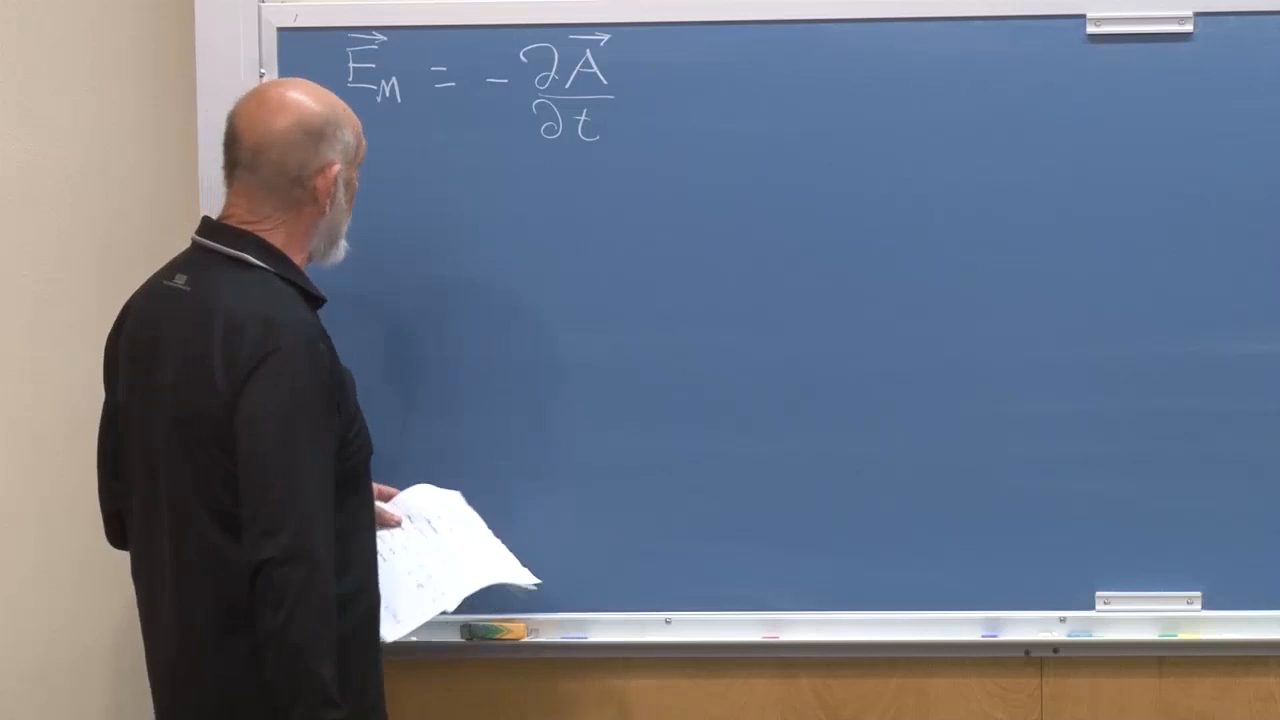
\includegraphics[width=\linewidth]{lecture_10_figure_02.png}\caption{Introduction de la quantité de mouvement mécanique comme le produit de la masse par la vitesse du centre de masse.}\par\smallskip
\textit{Image de la leçon : 00:11:15.}\end{figure}

\subsection{Quantité de mouvement canonique}

Supposons que la mécanique soit décrite par \(L(q_i,\dot q_i)\). La quantité de mouvement canonique conjuguée à \(q_i\) est \begin{equation}
p_i=\frac{\partial L}{\partial\dot q_i}.
\label{eq:canonical-momentum}
\end{equation} Pour \begin{equation}
L=\frac12 m\dot{\mathbf x}^{\,2}-V(\mathbf x),
\label{eq:simple-particle-lagrangian}
\end{equation}, on obtient \(\mathbf p=m\dot{\mathbf x}\) : les quantités de mouvement canonique et mécanique coïncident donc dans ce cas.

\begin{figure}[H]\centering
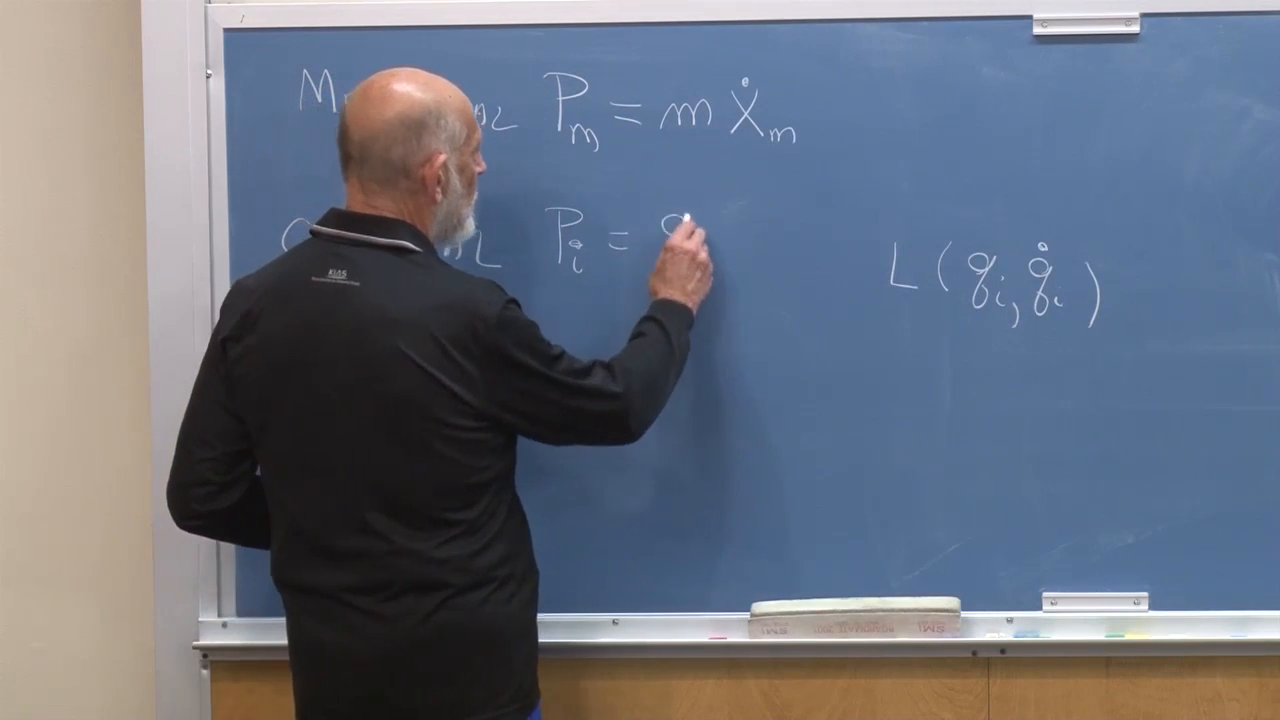
\includegraphics[width=\linewidth]{lecture_10_figure_03.png}\caption{Les quantités de mouvement mécanique et canonique présentées à côté du lagrangien simple d’une particule.}\par\smallskip
\textit{Image de la leçon : 00:13:40.}\end{figure}

Une particule chargée dans un champ magnétique fournit un contre-exemple utile. Avec la convention de signe inscrite au tableau, \begin{equation}
L=\frac12m\dot{\mathbf x}^{\,2}-V(\mathbf x)
  -e\,\dot{\mathbf x}\cdot\mathbf A(\mathbf x),
\label{eq:magnetic-particle-lagrangian}
\end{equation}, et donc \begin{equation}
p_i=m\dot x_i-eA_i.
\label{eq:magnetic-canonical-shift}
\end{equation}. Modifier la convention de signe de la charge ou celle du terme d’interaction change le signe affiché, mais pas la leçon à retenir : la quantité de mouvement canonique comporte une contribution du potentiel vecteur et ne se réduit pas à \(m\dot x_i\). Les équations de Hamilton font intervenir la variable canonique. On peut ensuite déplacer le terme dépendant du champ de l’autre côté d’une équation et retrouver une accélération d’allure newtonienne, mais ce réarrangement ne change pas la définition.

\begin{figure}[H]\centering
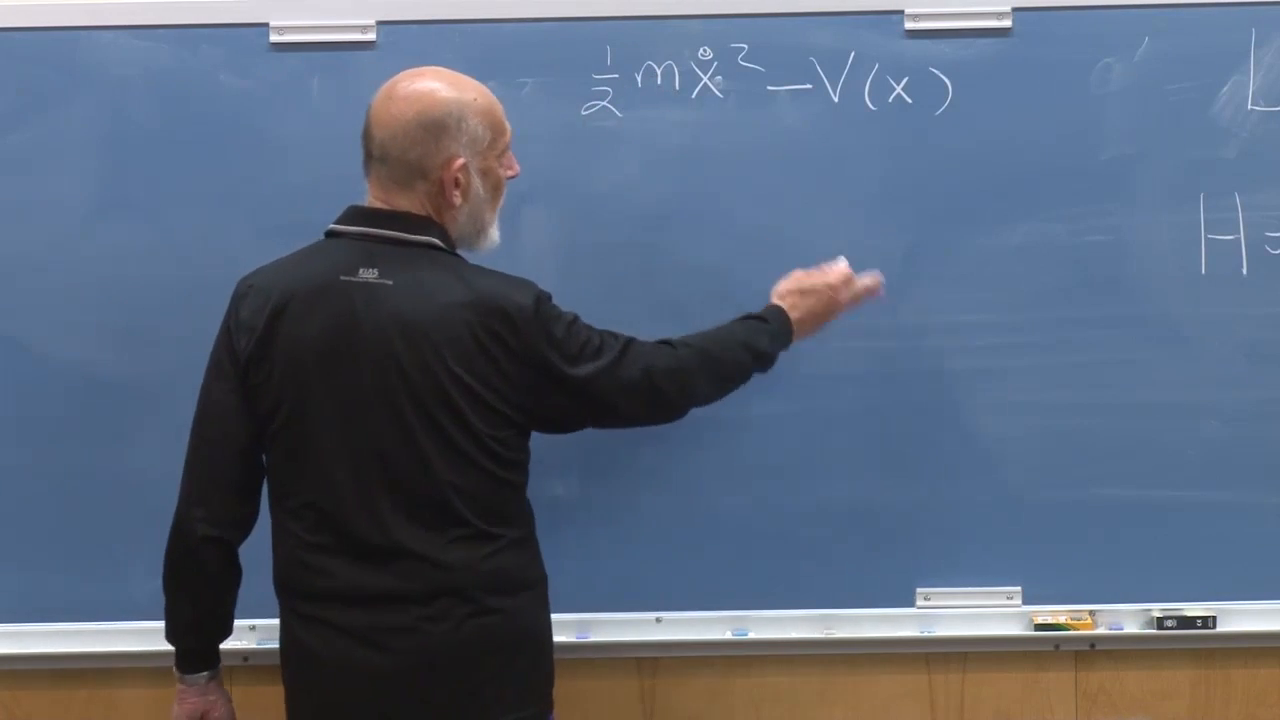
\includegraphics[width=\linewidth]{lecture_10_figure_04.png}\caption{Le terme de potentiel vecteur décale la quantité de mouvement canonique par rapport à la quantité de mouvement mécanique.}\par\smallskip
\textit{Image de la leçon : 00:15:50.}\end{figure}

\subsection{Quantité de mouvement de Noether}

La troisième quantité de mouvement est la charge conservée associée à l’invariance par translation spatiale. Pour une transformation infinitésimale \begin{equation}
q_i\longrightarrow q_i+\delta q_i
\end{equation} qui laisse le lagrangien invariant, le théorème de Noether donne, à la normalisation du paramètre infinitésimal près, \begin{equation}
Q=\sum_i p_i\,\delta q_i.
\label{eq:noether-charge-mechanics}
\end{equation} Les \(p_i\) qui apparaissent ici sont des quantités de mouvement canoniques. Si la symétrie est une translation uniforme et que la quantité de mouvement canonique coïncide avec la quantité de mouvement mécanique, \(Q\) se réduit à la quantité de mouvement totale usuelle. Dans un système moins simple, cette coïncidence doit être démontrée, et non supposée.

\begin{figure}[H]\centering
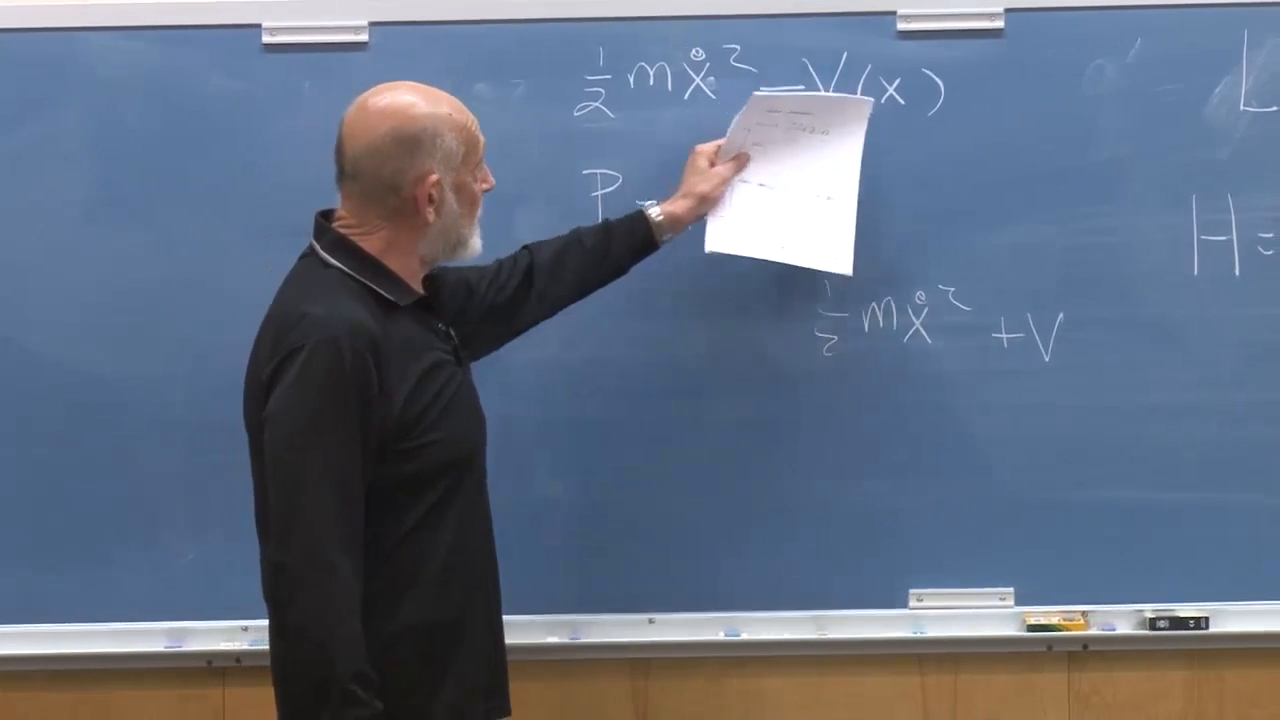
\includegraphics[width=\linewidth]{lecture_10_figure_05.png}\caption{Charge de Noether construite à partir des quantités de mouvement canoniques et des variations infinitésimales des coordonnées.}\par\smallskip
\textit{Image de la leçon : 00:19:00.}\end{figure}

\section{L’énergie comme hamiltonien}

Les translations spatiales conduisent à la quantité de mouvement ; les translations temporelles, à l’énergie. Si le lagrangien ne dépend pas explicitement du temps, le hamiltonien \begin{equation}
H=\sum_i p_i\dot q_i-L
\label{eq:hamiltonian-definition}
\end{equation} est conservé. C’est la transformée de Legendre du lagrangien, et non une règle permettant de changer les signes à vue.

\begin{figure}[H]\centering
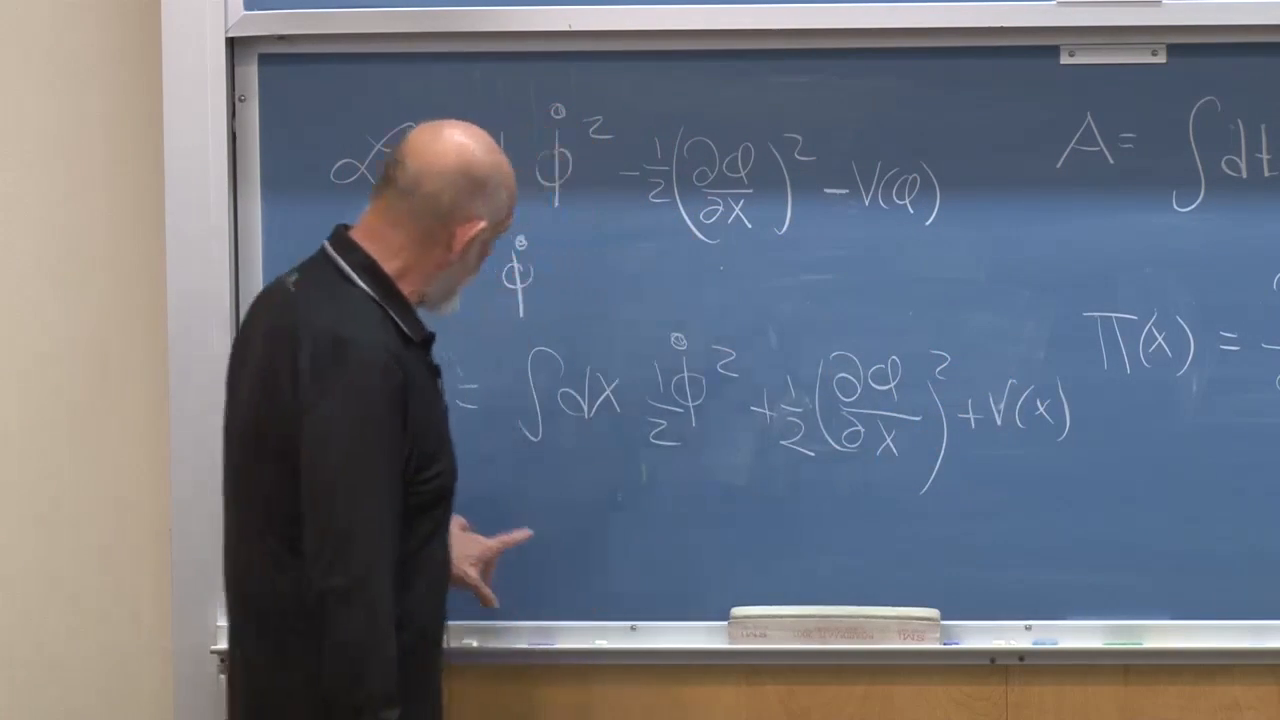
\includegraphics[width=\linewidth]{lecture_10_figure_06.png}\caption{Le hamiltonien écrit comme transformée de Legendre d’un lagrangien général.}\par\smallskip
\textit{Image de la leçon : 00:22:55.}\end{figure}

Pour l’exemple d’une particule, \begin{align}
p&=m\dot x,
\nonumber\\
H&=p\dot x-L\\
&=m\dot x^2
  -\left(\frac12m\dot x^2-V(x)\right)\\
&=\frac12m\dot x^2+V(x).
\label{eq:particle-hamiltonian}
\end{align}. Ainsi, le lagrangien est l’énergie cinétique moins l’énergie potentielle, tandis que le hamiltonien est l’énergie cinétique plus l’énergie potentielle.

\begin{figure}[H]\centering
\includegraphics[width=\linewidth]{lecture_10_figure_07.png}\caption{Le calcul pour la particule montre comment \(H=T+V\) découle de \(H=p\dot x-L\).}\par\smallskip
\textit{Image de la leçon : 00:24:20.}\end{figure}

Lorsque toute la dépendance en vitesse se présente sous la forme d’un terme cinétique quadratique positif usuel et que le reste ne dépend pas des vitesses, on peut lire le hamiltonien en changeant le signe de la partie indépendante des vitesses. Ce raccourci sera utilisé à plusieurs reprises. Il n’est valable que parce que, dans les exemples considérés, la transformée de Legendre prend cette forme simple.

\section{Un champ est un système mécanique à une infinité continue de coordonnées}

Pour mettre en évidence la structure mécanique de la théorie des champs, choisissons un référentiel inertiel et cessons provisoirement d’exiger que chaque ligne affiche manifestement la covariance de Lorentz. La mécanique classique comporte un axe temporel et des coordonnées \(q_i(t)\). Un champ scalaire comporte un axe temporel et des coordonnées \(\phi(\mathbf x,t)\). L’étiquette discrète \(i\) est simplement devenue l’étiquette continue \(\mathbf x\) : \begin{equation}
q_i(t)\quad\longrightarrow\quad\phi(\mathbf x,t).
\label{eq:discrete-to-field}
\end{equation} La valeur du champ en chaque point de l’espace constitue un degré de liberté. Ici, \(\mathbf x\) indique de quel degré de liberté il s’agit ; cette étiquette n’est pas elle-même la coordonnée généralisée.

\begin{figure}[H]\centering
\includegraphics[width=\linewidth]{lecture_10_figure_08.png}\caption{Réseau spatial représentant la valeur du champ en chaque point comme un degré de liberté mécanique distinct.}\par\smallskip
\textit{Image de la leçon : 00:30:15.}\end{figure}

\begin{classroomqa}\audiencequestion{Pourquoi ne pas écrire dès le départ le champ sous la forme \(\phi(\mathbf x,t)\)}\lecturerresponse{C’est la notation complète. La notation provisoire \(\phi(\mathbf x)\) omet l’argument temporel commun, comme on écrit souvent \(q_i\) en gardant à l’esprit que chaque \(q_i\) dépend du temps. L’étiquette \(i\), ou désormais \(\mathbf x\), indique le degré de liberté dont on parle. \lecturetimestamp{00:32:43}}\end{classroomqa}

\begin{classroomqa}\audiencequestion{Les valeurs du champ en des points voisins sont-elles vraiment des coordonnées indépendantes ? Qu’est-ce qui impose la continuité ?}\lecturerresponse{Ce sont des coordonnées canoniques indépendantes. La régularité n’est pas imposée en identifiant les valeurs voisines ; elle est sélectionnée par la dynamique. Le hamiltonien contient un terme d’énergie de gradient positif : un saut fixe sur une distance toujours plus petite coûte donc une énergie toujours plus grande. À la limite continue, les configurations d’énergie finie sont par conséquent régulières. \lecturetimestamp{00:33:09}}\end{classroomqa}

Une dérivée spatiale rend explicite le couplage entre degrés de liberté voisins. Sur un réseau d’espacement \(\epsilon\), \begin{equation}
\partial_x\phi(x,t)
  =\lim_{\epsilon\to0}
   \frac{\phi(x+\epsilon,t)-\phi(x,t)}{\epsilon}.
\label{eq:field-finite-difference}
\end{equation}. Elle dépend de deux coordonnées voisines, mais ne contient aucune vitesse généralisée. Dans l’analogie mécanique, elle relève de la dépendance du lagrangien en les coordonnées, et non de sa dépendance en \(\dot q_i\).

\begin{figure}[H]\centering
\includegraphics[width=\linewidth]{lecture_10_figure_09.png}\caption{Reconstitution de la dérivée spatiale comme différence entre les valeurs du champ en des points voisins du réseau.}\par\smallskip
\textit{Image de la leçon : 00:31:40.}\end{figure}

On peut maintenant écrire l’action sous une forme explicitement mécanique : \begin{align}
S&=\int dt\,L,
\nonumber\\
L&=\int d^3x\,
\mathcal L\!\left(
\phi,\dot\phi,\boldsymbol{\nabla}\phi
\right),
\nonumber\\
S&=\int dt\,d^3x\,
\mathcal L\!\left(
\phi,\dot\phi,\boldsymbol{\nabla}\phi
\right).
\label{eq:field-action-split}
\end{align} La lettre calligraphique \(\mathcal L\) désigne la densité lagrangienne ; son intégration sur l’espace donne le lagrangien ordinaire, qui est ensuite intégré sur le temps. Une théorie locale ne couple chaque point qu’au moyen des champs et de leurs dérivées en ce point. La séparation du temps et de l’espace masque momentanément la covariance de Lorentz, mais rend la structure mécanique transparente.

\begin{figure}[H]\centering
\includegraphics[width=\linewidth]{lecture_10_figure_10.png}\caption{Action du champ séparée en une intégrale temporelle et une intégrale spatiale de la densité lagrangienne.}\par\smallskip
\textit{Image de la leçon : 00:36:40.}\end{figure}

\section{Quantité de mouvement canonique du champ et densité hamiltonienne}

La vitesse d’une coordonnée de champ est \(\dot\phi(\mathbf x,t)\) : c’est le taux de variation temporelle du champ en un point fixe. Elle ne décrit pas un déplacement d’un point de l’espace à un autre. La quantité de mouvement canonique conjuguée au champ est donc elle-même un champ, \begin{equation}
\Pi(\mathbf x,t)
 =\frac{\partial\mathcal L}{\partial\dot\phi(\mathbf x,t)}.
\label{eq:field-canonical-momentum}
\end{equation} Pour plusieurs champs \(\phi_a\), il existe un champ de quantité de mouvement \(\Pi_a\) pour chacun d’eux.

La somme discrète dans la transformée de Legendre devient une intégrale spatiale : \begin{align}
H
 &=\int d^3x\,
   \left[\Pi\dot\phi-\mathcal L\right]
  =\int d^3x\,\mathcal H,
\nonumber\\
\mathcal H
 &=\Pi\dot\phi-\mathcal L .
\label{eq:field-hamiltonian-density}
\end{align} La quantité sous l’intégrale est la densité d’énergie.

\begin{figure}[H]\centering
\includegraphics[width=\linewidth]{lecture_10_figure_11.png}\caption{Transformée de Legendre du champ, interprétée comme une intégrale de la densité d’énergie locale.}\par\smallskip
\textit{Image de la leçon : 00:42:40.}\end{figure}

\begin{classroomqa}\audiencequestion{Pourquoi peut-on remplacer, en un point donné, la dérivée du lagrangien total par rapport à \(\dot\phi\) par celle de la densité locale ?}\lecturerresponse{Considérons l’intégrale spatiale comme une somme continue. Sous l’hypothèse de localité utilisée ici, la vitesse \(\dot\phi(\mathbf x)\) n’apparaît que dans le terme associé à ce même point. La dérivation par rapport à cette vitesse particulière élimine tous les autres termes. Les dérivées spatiales peuvent coupler les valeurs du champ en des points voisins, mais, dans cette théorie, elles n’introduisent pas de dérivées temporelles aux points voisins. \lecturetimestamp{00:51:56}}\end{classroomqa}

\subsection{Champ scalaire}

En une dimension spatiale, considérons \begin{equation}
\mathcal L
 =\frac12\dot\phi^2
  -\frac12(\partial_x\phi)^2
  -V(\phi).
\label{eq:scalar-field-lagrangian}
\end{equation} Il s’agit de l’écriture non covariante du scalaire de Lorentz introduit précédemment : le signe moins relatif entre les dérivées temporelle et spatiale provient de la métrique de Minkowski. La quantité de mouvement canonique est \begin{equation}
\Pi=\dot\phi,
\label{eq:scalar-pi}
\end{equation} et le hamiltonien devient \begin{equation}
H=\int dx\,
\left[
\frac12\dot\phi^2
+\frac12(\partial_x\phi)^2
+V(\phi)
\right].
\label{eq:scalar-field-hamiltonian}
\end{equation} Pendant le calcul, le potentiel a été momentanément noté \(V(x)\) ; la classe a corrigé cette notation en \(V(\phi)\). Il peut dépendre indirectement de la position par l’intermédiaire du champ, mais, dans la théorie invariante par translation, il ne dépend pas explicitement de \(x\).

\begin{figure}[H]\centering
\includegraphics[width=\linewidth]{lecture_10_figure_12.png}\caption{Densité lagrangienne scalaire, quantité de mouvement conjuguée et hamiltonien positif réunis au tableau.}\par\smallskip
\textit{Image de la leçon : 00:47:05.}\end{figure}

Toute la partie sans dérivées temporelles joue le rôle de l’énergie potentielle. Elle comprend à la fois \(V(\phi)\) et l’énergie de gradient \(\frac12(\partial_x\phi)^2\). Le lagrangien peut être de l’un ou l’autre signe ; une énergie stable doit être minorée.

\begin{classroomqa}\audiencequestion{Le potentiel \(V(\phi)\) peut-il être négatif ?}\lecturerresponse{Oui. S’il est minoré, on peut lui ajouter une constante de façon que son minimum soit nul, sans modifier l’équation classique du champ. Un potentiel non minoré décrit une instabilité : le champ peut abaisser son énergie sans limite. Le vide stable est un champ constant situé au minimum du potentiel décalé. \lecturetimestamp{00:49:03}}\end{classroomqa}

La question de continuité posée précédemment reçoit maintenant une réponse quantitative. Un saut \(\Delta\phi\) sur un espacement de réseau \(\epsilon\) contribue \begin{equation}
\frac12(\partial_x\phi)^2
\sim\frac12\left(\frac{\Delta\phi}{\epsilon}\right)^2.
\label{eq:gradient-cost}
\end{equation} Lorsque \(\epsilon\to0\), un saut fixe donne une densité d’énergie arbitrairement grande. Une énergie finie supprime donc les configurations irrégulières.

\begin{figure}[H]\centering
\includegraphics[width=\linewidth]{lecture_10_figure_13.png}\caption{La formule de l’énergie scalaire est conservée tandis que le schéma au tableau oppose un champ régulier à une variation brusque.}\par\smallskip
\textit{Image de la leçon : 00:54:20.}\end{figure}

\section{Énergie locale et signification de \texorpdfstring{\(T^{00}\)}{T00}}

La densité d’énergie reçoit une notation compacte : \begin{equation}
T^{00}=\mathcal H=\Pi\dot\phi-\mathcal L.
\label{eq:T00-definition}
\end{equation} Les deux indices nuls encodent deux énoncés distincts. L’énergie est la composante temporelle \(P^0\) du quadrivecteur énergie--quantité de mouvement, tandis qu’une densité est la composante temporelle d’un courant conservé. Ainsi, \(T^{00}\) est la densité de la composante temporelle du quadrivecteur énergie-quantité de mouvement.

\begin{figure}[H]\centering
\includegraphics[width=\linewidth]{lecture_10_figure_14.png}\caption{Énergie du champ écrite localement et identifiée à \(T^{00}\).}\par\smallskip
\textit{Image de la leçon : 01:00:00.}\end{figure}

Dans une théorie relativiste locale, la conservation ne signifie pas simplement qu’une grandeur globale reste inchangée. L’énergie ne peut pas disparaître du laboratoire et réapparaître à Alpha du Centaure. Toute variation dans une région doit s’expliquer par un flux traversant sa frontière. Sous forme locale, \begin{equation}
\partial_\mu T^{\mu\nu}=0,
\label{eq:stress-energy-continuity}
\end{equation} le premier indice désigne donc la densité ou la direction du flux, et le second indique quelle composante \(P^\nu\) est transportée.

\begin{classroomqa}\audiencequestion{Dire que \(T^{00}\) est une densité signifie-t-il qu’on obtient l’énergie totale en l’intégrant ?}\lecturerresponse{Exactement : \(E=P^0=\int d^3x\,T^{00}\). La densité locale est l’intégrande dans la transformée de Legendre du champ. Toute variation en un point est compensée par un courant d’énergie entre points voisins. \lecturetimestamp{00:59:06}}\end{classroomqa}

\section{Densité de quantité de mouvement issue des translations spatiales}

Revenons à la formule de Noether, en remplaçant maintenant la somme discrète par une intégrale spatiale. Lors d’une petite translation dans la direction \(m\), le champ varie de \begin{equation}
\delta\phi
  =\phi(\mathbf x)-\phi(\mathbf x-\boldsymbol{\epsilon})
  =\epsilon^m\partial_m\phi+O(\epsilon^2),
\label{eq:translated-field-change}
\end{equation} pour la convention passive utilisée au tableau. Inverser le sens des translations actives et passives inverse le signe global ; le générateur physique est fixé une fois cette convention choisie. En mettant \(\epsilon^m\) en facteur, la quantité de mouvement de Noether prend la forme \begin{equation}
P_m\ \propto\ \int d^3x\,\Pi\,\partial_m\phi.
\label{eq:scalar-noether-momentum}
\end{equation}

\begin{figure}[H]\centering
\includegraphics[width=\linewidth]{lecture_10_figure_15.png}\caption{Profil du champ translaté et dérivée qui mesure sa variation infinitésimale.}\par\smallskip
\textit{Image de la leçon : 01:04:20.}\end{figure}

\begin{classroomqa}\audiencequestion{Pourquoi le déplacement infinitésimal \(\epsilon\) ne figure-t-il pas dans la formule de la quantité de mouvement ?}\lecturerresponse{La charge de Noether est d’abord obtenue comme proportionnelle à \(\epsilon\). La quantité de mouvement est définie comme le coefficient de ce paramètre de translation arbitraire ; on divise donc par \(\epsilon\). Multiplier une grandeur conservée par une constante fixe ne modifierait pas sa conservation, mais extraire le coefficient donne la normalisation usuelle. \lecturetimestamp{01:04:45}}\end{classroomqa}

\begin{classroomqa}\audiencequestion{L’intervalle de translation devient-il le \(dx\) de l’intégrale continue ?}\lecturerresponse{Ces deux éléments proviennent de limites différentes. La mesure \(dx\) vient du remplacement de la somme sur les degrés de liberté indexés par les points de l’espace par une intégrale. Le paramètre de translation \(\epsilon\) décrit l’opération de symétrie et est mis en facteur dans la charge de Noether correspondante. Tous deux sont infinitésimaux dans le raisonnement intermédiaire, mais jouent des rôles différents. \lecturetimestamp{01:05:16}}\end{classroomqa}

Dans la notation de la leçon, la densité de la composante \(m\) de la quantité de mouvement est \begin{equation}
T^{0m}=\Pi\,\partial_m\phi,
\label{eq:scalar-momentum-density}
\end{equation}, la convention de signe pour les translations étant implicite. Pour la théorie scalaire, \(\Pi=\dot\phi\) ; elle est donc proportionnelle à \(\dot\phi\,\partial_m\phi\).

\begin{figure}[H]\centering
\includegraphics[width=\linewidth]{lecture_10_figure_16.png}\caption{Densité de quantité de mouvement de Noether \(T^{0m}=\Pi\,\partial_m\phi\) inscrite au tableau.}\par\smallskip
\textit{Image de la leçon : 01:07:10.}\end{figure}

Il s’agit de la quantité de mouvement réellement portée par une onde. L’invariance par translation ne s’applique que si tout est translaté : champs, particules, sources et appareils. Une impulsion lumineuse absorbée par un panneau libre de se déplacer le fait reculer. Avec la lumière ordinaire, l’effet est minime ; un laser suffisamment puissant peut transférer assez de quantité de mouvement pour comprimer une petite cible. La quantité conservée est celle de l’ensemble formé par les particules et les champs.

\subsection{Qu’est-ce qui remplace l’équation de Newton ?}

L’équation d’Euler--Lagrange du champ, dérivée de l’équation ~\eqref{eq:scalar-field-lagrangian}, est \begin{equation}
\ddot\phi-\nabla^2\phi=-\frac{dV}{d\phi}.
\label{eq:scalar-equation-of-motion}
\end{equation} C’est l’analogue, pour la théorie des champs, de la loi de Newton.

\begin{figure}[H]\centering
\includegraphics[width=\linewidth]{lecture_10_figure_17.png}\caption{Équation du champ scalaire présentée à côté de son hamiltonien et de sa densité de quantité de mouvement.}\par\smallskip
\textit{Image de la leçon : 01:12:55.}\end{figure}

\begin{classroomqa}\audiencequestion{Qu’est-ce qui correspond à la loi de Newton pour un champ ?}\lecturerresponse{C’est l’équation d’Euler--Lagrange du champ. Ici, il s’agit d’une équation d’onde avec le terme de force \(-V'(\phi)\). Le rôle de \(m\ddot x=-V'(x)\) est joué par \(\ddot\phi-\nabla^2\phi=-V'(\phi)\). \lecturetimestamp{01:11:48}}\end{classroomqa}

\begin{classroomqa}\audiencequestion{Comment sait-on qu’un lagrangien de champ proposé est correct ? Faut-il déjà connaître l’équation du champ ?}\lecturerresponse{Les deux démarches sont possibles. Historiquement, on peut déduire les équations des expériences, puis chercher une action, comme ce fut le cas pour Newton et Maxwell. Dans la théorie moderne, on part souvent du contenu en champs, de la localité, des symétries et d’un petit nombre de termes admissibles ; on en déduit les équations, puis on teste leurs prédictions. Le scalaire présenté pourrait décrire un champ fondamental, mais il pourrait tout aussi bien décrire le déplacement transversal d’une corde dont l’action continue est dérivée à partir de ses particules constitutives. \lecturetimestamp{01:12:55}}\end{classroomqa}

\section{Champ électromagnétique en jauge temporelle}

Les composantes déjà trouvées, \(T^{00}\) et \(T^{0m}\), appartiennent au tenseur énergie--quantité de mouvement. Ses autres composantes décrivent les flux d’énergie et de quantité de mouvement. Ce tenseur servira plus tard de source du champ gravitationnel, mais l’électromagnétisme en fournit un exemple immédiat.

La coordonnée électromagnétique fondamentale est le quadripotentiel \(A_\mu\). La liberté de jauge permet la transformation \begin{equation}
A_\mu\longrightarrow A'_\mu=A_\mu+\partial_\mu S
\label{eq:gauge-transformation-lecture10}
\end{equation} sans modifier \(F_{\mu\nu}\). Choisissons \(S\) de sorte que \begin{equation}
\partial_tS=-A_0.
\label{eq:temporal-gauge-choice}
\end{equation} Par exemple, on peut intégrer \(A_0\) par rapport au temps en chaque point fixe de l’espace. La composante temporelle transformée s’annule alors : \begin{equation}
A'_0=A_0+\partial_tS=0.
\label{eq:temporal-gauge}
\end{equation} C’est la jauge temporelle. Elle retire \(A_0\) de la liste des coordonnées dynamiques, bien que la loi de Gauss demeure une contrainte et qu’une liberté de jauge résiduelle, indépendante du temps, subsiste.

\begin{figure}[H]\centering
\includegraphics[width=\linewidth]{lecture_10_figure_18.png}\caption{Liberté de jauge utilisée pour imposer \(A_0=0\) en résolvant \(\partial_tS=-A_0\).}\par\smallskip
\textit{Image de la leçon : 01:20:15.}\end{figure}

À partir de maintenant, notons \(\mathbf E\) le champ standard de Maxwell. Avant de fixer la jauge, \begin{equation}
E_m=-\partial_tA_m+\partial_mA_0,
\qquad
\mathbf B=\boldsymbol{\nabla}\times\mathbf A.
\label{eq:E-B-general-potential}
\end{equation} En jauge temporelle, ces relations se réduisent à \begin{equation}
\mathbf E=-\dot{\mathbf A},
\qquad
\mathbf B=\boldsymbol{\nabla}\times\mathbf A.
\label{eq:E-B-temporal-gauge}
\end{equation} Les dérivées temporelles de \(\mathbf A\) donnent le champ électrique ; les dérivées spatiales donnent le champ magnétique.

\begin{figure}[H]\centering
\includegraphics[width=\linewidth]{lecture_10_figure_19.png}\caption{Champs électrique et magnétique en jauge temporelle : \(\mathbf E=-\dot{\mathbf A}\) et \(\mathbf B=\nabla\times\mathbf A\).}\par\smallskip
\textit{Image de la leçon : 01:23:50.}\end{figure}

\section{Quantité de mouvement canonique et énergie électromagnétiques}

La densité lagrangienne de Maxwell dans le vide est \begin{equation}
\mathcal L_{\mathrm{EM}}
 =-\frac14F_{\mu\nu}F^{\mu\nu}
 =\frac12\left(\mathbf E^2-\mathbf B^2\right).
\label{eq:maxwell-lagrangian-energy-lecture}
\end{equation} En jauge temporelle, \begin{equation}
\mathcal L_{\mathrm{EM}}
 =\frac12\dot{\mathbf A}^{\,2}
  -\frac12(\boldsymbol{\nabla}\times\mathbf A)^2.
\label{eq:maxwell-lagrangian-temporal}
\end{equation} Elle présente exactement la structure du champ scalaire : les carrés des dérivées temporelles moins ceux des dérivées spatiales.

\begin{figure}[H]\centering
\includegraphics[width=\linewidth]{lecture_10_figure_20.png}\caption{Le lagrangien de Maxwell réécrit sous forme d’un lagrangien mécanique de champ pour les composantes spatiales de \(\mathbf A\).}\par\smallskip
\textit{Image de la leçon : 01:28:10.}\end{figure}

Chaque composante \(A_m\) possède une quantité de mouvement canonique, \begin{equation}
\Pi_m
 =\frac{\partial\mathcal L_{\mathrm{EM}}}
        {\partial\dot A_m}
 =\dot A_m
 =-E_m.
\label{eq:em-canonical-momentum}
\end{equation}. Voilà un exemple concret de l’importance d’une convention. Avec la convention antérieure, où le champ électrique avait le signe opposé, le signe final affiché changerait, même si la dérivée canonique elle-même resterait inchangée.

\begin{figure}[H]\centering
\includegraphics[width=\linewidth]{lecture_10_figure_21.png}\caption{Les trois champs de quantité de mouvement canonique associés à \(A_x,A_y,A_z\), chacun égal à la dérivée temporelle correspondante et donc à l’opposé du champ électrique standard.}\par\smallskip
\textit{Image de la leçon : 01:30:20.}\end{figure}

Le raccourci pour calculer le hamiltonien est maintenant justifié : on change le signe du terme sans dérivées temporelles. La densité d’énergie électromagnétique est \begin{equation}
T^{00}_{\mathrm{EM}}
 =\mathcal H_{\mathrm{EM}}
 =\frac12\left(\mathbf E^2+\mathbf B^2\right),
\label{eq:em-energy-density}
\end{equation} et \begin{equation}
H_{\mathrm{EM}}
 =\int d^3x\,
\frac12\left(\mathbf E^2+\mathbf B^2\right).
\label{eq:em-total-energy}
\end{equation} Contrairement à la densité lagrangienne, la densité d’énergie est non négative.

\begin{figure}[H]\centering
\includegraphics[width=\linewidth]{lecture_10_figure_22.png}\caption{Densité hamiltonienne électromagnétique positive \(\frac12(\mathbf E^2+\mathbf B^2)\).}\par\smallskip
\textit{Image de la leçon : 01:32:00.}\end{figure}

Pour une onde plane dans le vide, \(\mathbf E\perp\mathbf B\), les deux champs sont en phase et, en unités où \(c=1\), ils ont même amplitude. Les contributions électrique et magnétique se partagent donc également l’énergie de l’onde : \begin{equation}
u_E=\frac12\mathbf E^2,
\qquad
u_B=\frac12\mathbf B^2,
\qquad
u_E=u_B.
\label{eq:plane-wave-energy-halves}
\end{equation}

\section{Dérivation de la quantité de mouvement électromagnétique}

Il faut maintenant sommer la formule de translation de Noether sur les trois champs \(A_m\). En choisissant le signe de la translation de façon que la quantité de mouvement physique pointe dans le sens de propagation de l’onde, la composante \(n\) est \begin{equation}
P_n
 =\int d^3x\,E_m\,\partial_nA_m,
\label{eq:em-canonical-noether-momentum}
\end{equation} où la sommation porte sur \(m\). La leçon s’arrête délibérément sur la question du signe : il dépend des choix précédemment faits pour le champ électrique et pour les translations actives ou passives. Le résultat physique, invariant de jauge, permettra de le fixer.

\begin{figure}[H]\centering
\includegraphics[width=\linewidth]{lecture_10_figure_23.png}\caption{Formule de Noether pour le champ scalaire étendue aux trois composantes du potentiel vecteur.}\par\smallskip
\textit{Image de la leçon : 01:36:40.}\end{figure}

L’intégrande contient encore le potentiel de jauge, et pas uniquement les champs physiques. Ajoutons et retranchons \(E_m\partial_mA_n\) : \begin{align}
E_m\partial_nA_m
 &=
 E_m\left(\partial_nA_m-\partial_mA_n\right)
 +E_m\partial_mA_n.
\label{eq:add-subtract-em-momentum}
\end{align} Le premier terme est un produit vectoriel, \begin{equation}
E_m\left(\partial_nA_m-\partial_mA_n\right)
  =(\mathbf E\times\mathbf B)_n.
\label{eq:cross-product-component}
\end{equation} Le second s’intègre par parties : \begin{align}
\int d^3x\,E_m\partial_mA_n
 &=
\int_{\partial V}d\Sigma_m\,E_mA_n
-\int d^3x\,A_n\partial_mE_m.
\label{eq:em-momentum-integration-parts}
\end{align} Si les champs décroissent suffisamment vite pour que le terme de bord s’annule, et si la région est dépourvue de sources, de sorte que \(\boldsymbol{\nabla}\cdot\mathbf E=0\), le second terme ne contribue pas.

\begin{figure}[H]\centering
\includegraphics[width=\linewidth]{lecture_10_figure_24.png}\caption{Le terme ajouté, transféré à \(\nabla\cdot\mathbf E\) par intégration par parties.}\par\smallskip
\textit{Image de la leçon : 01:40:00.}\end{figure}

La quantité de mouvement totale du champ est donc \begin{equation}
\mathbf P_{\mathrm{EM}}
 =\int d^3x\,\mathbf E\times\mathbf B,
\qquad
\mathbf g_{\mathrm{EM}}
 =\mathbf E\times\mathbf B,
\label{eq:em-momentum-density}
\end{equation} dans les unités utilisées dans la leçon. Le vecteur \(\mathbf g_{\mathrm{EM}}\) est la densité de quantité de mouvement électromagnétique.

\begin{figure}[H]\centering
\includegraphics[width=\linewidth]{lecture_10_figure_25.png}\caption{L’expression en potentiel de jauge réduite à la quantité de mouvement invariante de jauge \(\int d^3x\,\mathbf E\times\mathbf B\).}\par\smallskip
\textit{Image de la leçon : 01:41:10.}\end{figure}

\begin{classroomqa}\audiencequestion{Où a-t-on utilisé \(\boldsymbol{\nabla}\cdot\mathbf E=0\), et que se passe-t-il en présence de charges ?}\lecturerresponse{Cette condition élimine le terme de volume après intégration par parties ; la dérivation présentée, qui ne fait intervenir que le champ, s’applique donc à une onde électromagnétique libre. En présence de charges, ce terme n’est pas nul et il faut inclure la quantité de mouvement de la matière chargée. L’invariance par translation et la conservation de la quantité de mouvement concernent l’ensemble du système matière--champ. \lecturetimestamp{01:41:55}}\end{classroomqa}

\subsection{Direction de la quantité de mouvement de l’onde}

Dans une onde plane, \(\mathbf E\), \(\mathbf B\) et la direction de propagation forment un trièdre direct. Une demi-longueur d’onde plus loin, \(\mathbf E\) et \(\mathbf B\) changent tous deux de sens : \begin{equation}
(-\mathbf E)\times(-\mathbf B)
 =\mathbf E\times\mathbf B.
\label{eq:poynting-sign-reversal}
\end{equation} La densité de quantité de mouvement pointe donc toujours dans une direction fixe au cours de l’oscillation, celle de la propagation de l’onde.

\begin{figure}[H]\centering
\includegraphics[width=\linewidth]{lecture_10_figure_26.png}\caption{Géométrie de l’onde plane : les champs électrique et magnétique s’inversent ensemble, tandis que leur produit vectoriel reste dirigé selon l’axe de propagation.}\par\smallskip
\textit{Image de la leçon : 01:43:10.}\end{figure}

C’est pourquoi la pression de radiation est bien réelle. L’absorption transfère la quantité de mouvement du champ à la matière ; la réflexion inverse la quantité de mouvement de la lumière et peut transférer au réflecteur deux fois sa composante normale.

\section{Quand le potentiel rencontre les champs observables}

À la fin du cours, la classe demande quels sont les liens entre \(A_\mu\) et les champs observables. Ce sont précisément les relations suivantes :
\begin{align}
E_n&=-\partial_tA_n+\partial_nA_0,
\nonumber\\
B_n&=\epsilon_{nmk}\partial_mA_k.
\label{eq:potential-field-contact}
\end{align}
La jauge temporelle élimine le terme \(A_0\), sans modifier les champs physiques.

\begin{figure}[H]
\centering
\includegraphics[width=\linewidth]{lecture_10_figure_27.png}
\caption{La relation générale entre le champ électrique et le potentiel, rétablie après le calcul en jauge temporelle, ainsi que le lagrangien scalaire covariant rappelé en dessous.}
\par\smallskip
\textit{Cadre de la leçon : 01:45:40.}
\end{figure}

\begin{classroomqa}
\audiencequestion{Quel est le lien exact entre le potentiel vecteur et les champs électrique et magnétique ?}
\lecturerresponse{Le champ électrique combine la dérivée temporelle du potentiel spatial et la dérivée spatiale de \(A_0\) ; le champ magnétique est le rotationnel du potentiel spatial. En jauge temporelle, on obtient simplement
\(\mathbf E=-\dot{\mathbf A}\) et
\(\mathbf B=\nabla\times\mathbf A\).
\lecturetimestamp{01:44:15}}
\end{classroomqa}

\begin{classroomqa}
\audiencequestion{Le potentiel est-il plus fondamental que \(\mathbf E\) et \(\mathbf B\) ?}
\lecturerresponse{L’action et le principe de jauge se formulent le plus naturellement à l’aide de \(A_\mu\), ce qui confère au potentiel un rôle fondamental dans la structure de la théorie. Pourtant, \(A_\mu\) n’est pas unique : des potentiels reliés par une transformation de jauge décrivent la même physique, et les champs locaux sont invariants de jauge. Ces deux affirmations sont compatibles. Les variables fondamentales ne sont pas nécessairement directement observables. \lecturetimestamp{01:46:36}}
\end{classroomqa}

\begin{classroomqa}
\audiencequestion{Le potentiel de jauge lui-même peut-il exercer une force ?}
\lecturerresponse{Un représentant dépendant de la jauge ne peut pas produire de force mesurable qui dépende de la jauge. La matière chargée est couplée au potentiel dans l’action, mais la force de Lorentz classique peut s’exprimer entièrement à l’aide des champs électrique et magnétique, qui sont invariants de jauge.
\lecturetimestamp{01:47:49}}
\end{classroomqa}

\begin{classroomqa}
\audiencequestion{Si des champs électrique et magnétique croisés sont statiques, leur quantité de mouvement doit-elle être nulle ?}
\lecturerresponse{Pas nécessairement pour le champ seul :
\(\mathbf E\times\mathbf B\) peut être non nul même si les deux champs sont indépendants du temps. Dans un dispositif statique fermé, le bilan complet de la quantité de mouvement inclut aussi les charges, les courants, les supports ainsi que toute quantité de mouvement mécanique ou cachée. La brève réponse donnée en classe — le total doit s’équilibrer — exprime correctement la conservation ; imposer une contribution nulle du champ seul serait aller trop loin.
\lecturetimestamp{01:48:01}}
\end{classroomqa}

\section{Un tenseur, deux sens du vecteur de Poynting}

Le tenseur énergie--impulsion rassemble toutes les densités et tous les flux :
\begin{align}
T^{00}&=\text{energy density},\\
T^{0i}&=\text{\(i\)-momentum density},\\
T^{i0}&=\text{energy flux in the \(i\)-direction},\\
T^{ij}&=\text{\(j\)-momentum flux in the \(i\)-direction}.
\label{eq:stress-energy-components}
\end{align}
Par exemple, \(T^{31}\) représente la quantité de \(x\)-impulsion qui traverse, par unité de temps, une unité de surface dont la normale est orientée dans la direction \(z\). Le bloc spatial \(T^{ij}\) est le tenseur des contraintes.

\begin{figure}[H]
\centering
\includegraphics[width=\linewidth]{lecture_10_figure_28.png}
\caption{Au tableau, les composantes de densité et de flux commencent à être rassemblées dans le tenseur énergie--impulsion.}
\par\smallskip
\textit{Cadre de la leçon : 01:51:10.}
\end{figure}

Pour les systèmes relativistes considérés ici, on peut choisir le tenseur énergie--impulsion physique de sorte qu’il soit symétrique :
\begin{equation}
T^{\mu\nu}=T^{\nu\mu}.
\label{eq:stress-energy-symmetry}
\end{equation}
Par conséquent,
\begin{equation}
T^{0i}=T^{i0}.
\label{eq:momentum-density-energy-flux}
\end{equation}
La densité de \(i\)-impulsion est égale au flux d’énergie dans la direction \(i\) lorsque \(c=1\). Voilà la réponse à la dernière question du public : le vecteur de Poynting est bien une densité de puissance.

\begin{classroomqa}
\audiencequestion{\(\mathbf E\times\mathbf B\) est-il une densité de puissance plutôt qu’une densité de quantité de mouvement ?}
\lecturerresponse{C’est les deux. La symétrie de \(T^{\mu\nu}\) identifie la densité de quantité de mouvement \(T^{0i}\) au flux d’énergie \(T^{i0}\). Ainsi, \(\mathbf S=\mathbf E\times\mathbf B\) représente une énergie par unité de temps et par unité de surface et, en \(c=1\), une quantité de mouvement par unité de volume. Lorsque l’on rétablit les unités usuelles, \(\mathbf g=\mathbf S/c^2\).
\lecturetimestamp{01:48:20}}
\end{classroomqa}

\begin{figure}[H]
\centering
\includegraphics[width=\linewidth]{lecture_10_figure_29.png}
\caption{La relation de symétrie du tenseur, qui égalise la densité de quantité de mouvement et le flux d’énergie, est désignée au tableau par le vecteur de Poynting.}
\par\smallskip
\textit{Cadre de la leçon : 01:53:50.}
\end{figure}

\section{Le pont vers la relativité générale}

Le cours s’achève en réunissant la mécanique classique, la théorie des champs et l’électromagnétisme dans une même structure :
\begin{enumerate}
\item L’invariance par translation temporelle donne le hamiltonien et l’énergie.
\item L’invariance par translation spatiale donne la quantité de mouvement de Noether.
\item Le remplacement des coordonnées discrètes par des champs repérés dans l’espace transforme les sommes en intégrales et les quantités conservées en densités locales.
\item La fixation de jauge fait apparaître les coordonnées mécaniques du champ de Maxwell sans modifier ses observables.
\item L’hamiltonien de Maxwell donne
\(\frac12(\mathbf E^2+\mathbf B^2)\), tandis que les translations spatiales donnent
\(\mathbf E\times\mathbf B\).
\item Le tenseur énergie--impulsion symétrique unifie la densité d’énergie, la densité de quantité de mouvement, le flux d’énergie et les contraintes.
\end{enumerate}

C’est la grandeur dont on aura besoin à l’étape suivante. En relativité générale, le tenseur énergie--impulsion apparaît comme source dans l’équation de champ d’Einstein. La dernière leçon ne s’est donc pas contentée d’ajouter un calcul électromagnétique : elle a préparé le langage qui permet à la matière et aux champs de dire à l’espace-temps comment se courber.
